\section{A Grounded Agentic Diagnostician}
\label{sec:system}

The object we build is an agent that answers questions about a generated
parallel program the way a grounded model-explanation answers questions about a
prediction: by calling tools that return real measurements, and by saying
nothing the tools did not return. It has two roles, and a discipline that binds
both (Figure~\ref{fig:architecture}).

\begin{figure}[t]
\centering
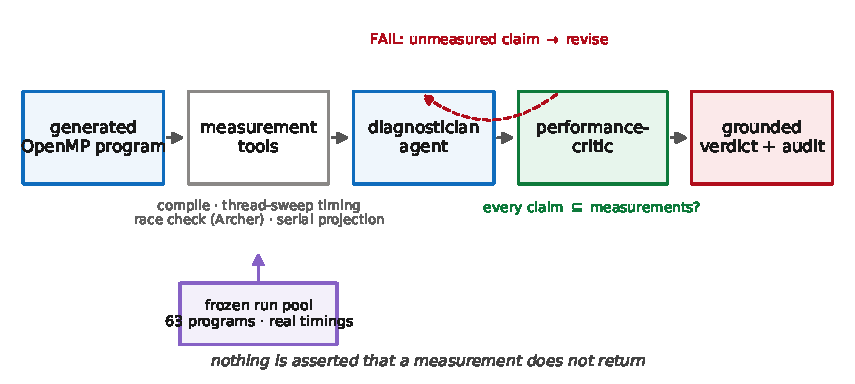
\includegraphics[width=\columnwidth]{figs/architecture}
\caption{The grounded agentic diagnostician. The agent may call only measurement
tools - compile, thread-count sweep timing, an independent race check, and the
serial projection - over a frozen pool of executed programs; the
performance-critic fails any drafted claim not entailed by those measurements and
returns it for revision. The same efficiency gate the critic enforces at
inference (Section~\ref{sec:reward}) is the reward a post-training loop should
optimize - the checker and the reward are one object.}
\label{fig:architecture}
\end{figure}

\paragraph*{Tools, not assertions}
The diagnostician is a tool-calling LLM over a fixed set of
measurement tools, each of which reports a fact about a program that was
actually compiled and run: its correctness at every thread count in the sweep
$\{1,2,4,8\}$; its per-thread wall-times and the resulting self-speedup
$S(p)=T(1)/T(p)$ and efficiency $S(p)/p$; its speedup against the trusted serial
reference; the race verdict from an independent happens-before detector; the
synchronization idiom it used; and the \emph{\SP} - the source with every
OpenMP directive deleted - together with the reward each formulation pays it.
The agent chooses which tools to call and narrates their results; it is
forbidden, by system prompt and by the critic below, from stating a speedup, a
race verdict, or a ``correct but not parallel'' judgement that no tool returned.
This is the parallel-code analogue of never inventing a feature attribution: a
diagnosis is admissible only if a measurement backs every number in it.

\paragraph*{The performance-critic}
A second agent re-reads the tool outputs - the only source of truth - and the
draft diagnosis, and fails any claim the measurements do not support: an
invented speedup, a race the detector did not find, or an assertion of scaling
where none was measured. It is the acceptance gate the naive agent lacks. A
correctness-only self-acceptance loop terminates when the output matches the
reference, which (Section~\ref{sec:degeneracy}) it does for programs that are
correct and serial; the performance-critic terminates only when the measured
efficiency, not just the output, is what it claims. The rest of this paper is
the argument for why that second gate is necessary and how it should be shaped:
the degeneracy of the output-only gate (Section~\ref{sec:degeneracy}), the
efficiency-gated reward the critic enforces (Section~\ref{sec:reward}), and its
behaviour under adversarial attack (Section~\ref{sec:results-hacks}).

\paragraph*{Why not just a general agent}
It is fair to ask what a general tool-using agent, handed a compiler and a timer,
would do differently - and the answer is the paper's thesis in miniature. A
general agent decides a draft is finished the way agents do: it runs the program
and checks the output against the reference. Proposition~\ref{prop:degeneracy} is
precisely the statement that this stopping rule is degenerate, satisfied
maximally by the program with every \texttt{\#pragma omp} deleted. Such an agent
does not do what ours does; it does the exact thing we prove is wrong, and it
does so confidently, because from the output side a serial program is
indistinguishable from a parallel one. The distinction is not that our agent is
smarter but that its \emph{gate} is different, in three ways. Its stop condition
is measured strong-scaling efficiency against the trusted reference - a physical
wall time a serial program cannot fake - rather than output-equivalence. Its
claims are grounded by construction: the performance-critic fails any parallelism
assertion no tool returned, so unlike a general agent it cannot pass a speedup it
never measured. And the very gate it enforces at inference is, unchanged, the
verifiable reward for post-training (Section~\ref{sec:reward}), so the pipeline
from generation through differential correctness, reference-anchored timing, race
checking, and the serial projection down to the efficiency gate is
\emph{end-to-end}: its verdict serves at once as the agent's acceptance test and
as the training signal. A general agent gives you the front of that pipe and
halts at the point we show is wrong. The novelty is therefore not the agent's
machinery, which is ordinary tool calling, but three things a general agent has
no reason to include: a stop condition grounded in a measurement it cannot fake,
a critic that refuses any claim no tool returned, and the identity between that
inference-time gate and the post-training reward.

\paragraph*{A diagnosis, grounded}
Asked for the worst-scaling accepted program, the agent calls the read tool and
reports: task \texttt{histogram\_bin\_0-100}, correct at every thread count and
race-clean, yet self-speedup \emph{0.33}$\times$ at 8 threads (efficiency
0.04) - slower than serial. Correctness-only reward: \emph{1.0}, identical to a
program that scales to \SpeedMax$\times$; efficiency-gated reward:
\emph{0.04}. Two programs the verifier certified equally correct on this one
task span \WorstTaskRange$\times$. Every number in that paragraph is a tool
return, and the critic passes it because every number is; strip the measurements
and the agent has nothing to say, which is the point. The remainder of the paper
measures, on a frozen pool of \NAccepted\ programs, exactly what that grounding
buys.
